\chapter{\label{chap:intro}Introdução}

Em 2014, 54\% da população mundial vivia em áreas urbanas, de acordo com a Organização das Nações Unidas (\cite{UN14}). A expectativa é que esta proporção aumente para 66\% até o ano 2050. Em números absolutos isto representa um acréscimo de 2,5 bilhões de pessoas à população urbana mundial nos próximos 35 anos. Uma das consequências da alta densidade populacional em regiões geográficas limitadas é o crescimento do modelo de verticalização na construção civil. Neste cenário, onde prédios de diversos andares se tornam presença no cotidiano da maioria da população, os elevadores passam a um papel de grande destaque.

Uma pesquisa realizada pela IBM no ano de 2010 (\cite{HORN10}) em 16 cidades norte-americanas constatou que, durante 12 meses, o tempo acumulado no qual trabalhadores de escritórios aguardaram por elevadores foi de absurdos 92 anos. Em uma economia onde o salário horário médio de um trabalhador é de US\$ 24,99 (\cite{BLS15}), o tempo de espera por elevadores representa um prejuízo de mais de US\$ 20.000.000 em média por ano.

Além do impacto econômico existe o impacto psicológico. Trabalhadores de grandes cidades empreendem uma grande parcela da sua rotina no deslocamento entre residência e local de trabalho e no caminho inverso ao final do dia. Além de gastar uma quantidade significativa de tempo no trânsito das ruas, em carros, ônibus, bicicletas e metrôs, o tempo compreendido entre aguardar o elevador e desembarcar no andar desejado está longe de ser desprezível. São momentos que a pessoa poderia utilizar para outros fins, como produzir (trabalhar), relaxar, jantar com a esposa, brincar com os filhos, etc. {\color{red}[BUSCAR FONTES PARA ESTE PARÁGRAFO]}

\begin{figure}[htb!]
\centering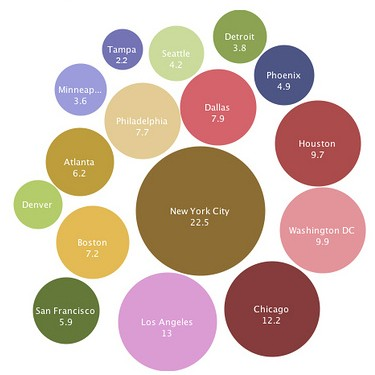
\includegraphics{img/time-cost.jpg}
\caption{\label{fig:fig1}Tempo de espera acumulado (em anos) por elevadores durante 12 meses em 16 cidades norte-americanas. Fonte: \cite{HORN10}}
\end{figure}

Neste contexto global, a indústria de elevadores possui grandes desafios: primeiro, lidar com a pressão para a redução de custos na construção civil, construindo elevadores menores e com melhorias no desempenho de transporte; segundo, competir no mercado oferecendo serviços novos, personalizados e com garantia de qualidade, visando revolucionar a maneira com que elevadores interagem e servem passageiros (\cite{KOEHLEROTTIGER02}). Para ajudar a atingir estes objetivos, fabricantes de elevadores vem estudando e aplicando desde meados dos anos 1980 diversas técnicas de Inteligência Artificial. Técnicas como redes neurais, algoritmos genéticos, lógicas \textit{fuzzy} e, mais recentemente, sistemas multi-agentes e planejamento foram adotados pela indústria.

\section{Motivação prática}
\section{Testar conhecimentos}
\subsection{IA}
\subsection{Programação}
\section{Simulação}